130. \begin{figure}[ht!]
\center{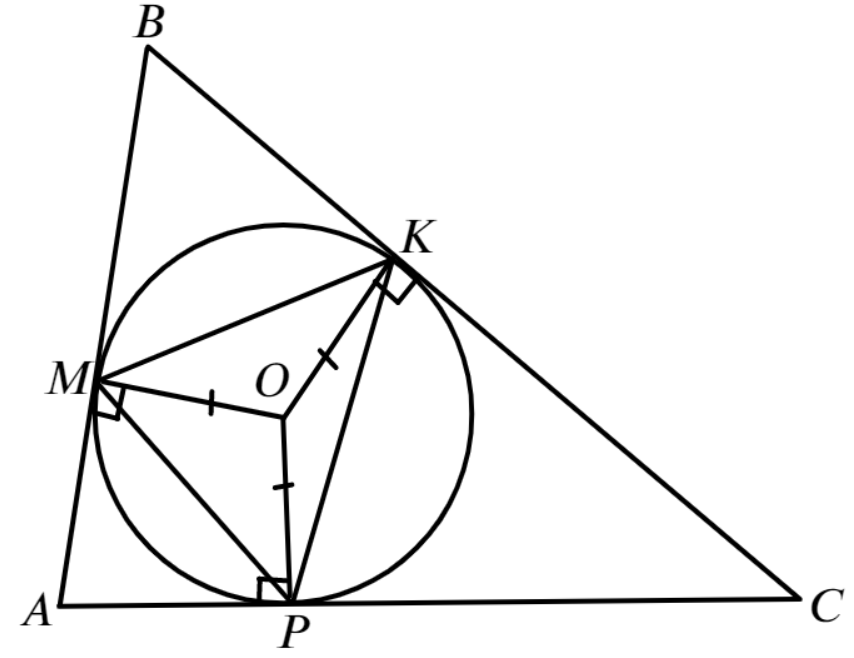
\includegraphics[scale=0.35]{g9-130.png}}
\end{figure}\\
Пусть $\angle A=2x,\ \angle B=2y,\ \angle C=2z.$ Тогда выразим из четырёхугольников $AMOP,\ BMOK,\ CKOP$ углы: $\angle MOP=360^\circ-90^\circ-90^\circ-x=180^\circ-2x$ и аналогично $\angle MOK=180^\circ-2y,\ \angle KOP=180^\circ-2z.$ Так как треугольники $MOP,\ MOK$ и $KOP$ являются равнобедренными, выразим углы $\angle OMP=\angle OPM=x,\ \angle OMK=\angle OKM=y,\ \angle OPK=\angle OKP=z.$ Тогда имеем систему уравнений $\begin{cases} x+y=56^\circ,\\ y+z=57^\circ,\\ z+x=67^\circ.\end{cases},$ откуда $x+y+z=\cfrac{56^\circ+57^\circ+67^\circ}{2}=90^\circ,\ x=90^\circ-57^\circ=33^\circ,\ y=90^\circ-67^\circ=23^\circ,\ z=90^\circ-56^\circ=34^\circ.$ Тогда углы треугольника $ABC$ равны $2\cdot33=66^\circ,\ 2\cdot23=46^\circ,\ 2\cdot34=68^\circ.$\\
